\section{Evaluation}
\label{sec:evaluation}

Cudele lets users construct consistency/durability guarantees using
well-established research techniques from other systems; so instead of
evaluating the scalability and performance of the techniques themselves against
other file systems, we show that (1) the mechanisms we propose are useful for
constructing semantics used by real systems, (2) the techniques can work
side-by-side in the same namespace, and (3) the combination of these techniques
can help the system scale further when subtrees are coupled to the correct type
of application.  We scope the evaluation to one metadata server and scale the
number of parallel clients. This type of analysis shows the capacity and
performance of a metadata server with superior metadata protocols, which should
be used to inform load balancing across a metadata cluster. Load balancing
across a cluster of metadata servers with partitioning and replication can be
explored with something like Mantle~\cite{sevilla:sc15-mantle}.

%\begin{table}
%\begin{tabular}{ r | l | l}
%  Cluster  & Hardware               & Software \\\hline
%  In-House & 15 nodes, 4 2GHz CPUs  & Ubuntu 12.04, 1 MON\\
%           & 8GB RAM, SSD           & 1 MDS, 8 OSDs, 8 Clients\\
%  CloudLab & 34 nodes, 16 2.4GHz CPUs & Ubuntu 14.04, 1 MON\\
%           & 128GB RAM, SSD         & 1 MDS, 3 OSDs, 29 Clients
%\end{tabular}
%\caption{In-House used for microbenchmarks, CloudLab for Use Cases. MON is
%monitor daemon, MDS is metadata server daemon, and OSDs are object storage
%daemons.\label{table:clusters}} 
%\end{table}

%We run experiments on the same cluster and normalize results to control for
%hardware differences and to make our results more generally applicable and
%reproducible\footnote{ This paper adheres to The Popper
%Convention~\cite{jimenez_popper_2016}, so experiments presented here are
%available in the repository for this article.  Experiments can be examined in
%more detail, or even re-run, by visiting the \texttt{[source]} link next to
%each figure. That link points to a Jupyter notebook that shows the analysis and
%source code for that graph, which points to an experiment and its artifacts.}.
%We use a CloudLab cluster of 34 nodes, each with 16 2.4 GHz CPUs, 128GB RAM,
%and SSDs.  Each node uses Ubuntu 14.04 and We develop on Ceph's Jewel release,
%version 10.2.1, which was released in May 2016. All daemons run as a single
%process (the default setting for Ceph) and the Ceph
%components\footnote{http://docs.ceph.com/docs/jewel/rados/} are: 1 monitor, 3
%object storage daemons, 1 metadata server, and 29 clients.

\subsection{Microbenchmarks}
\label{sec:microbenchmarks}
\begin{figure}[tb]
\centering
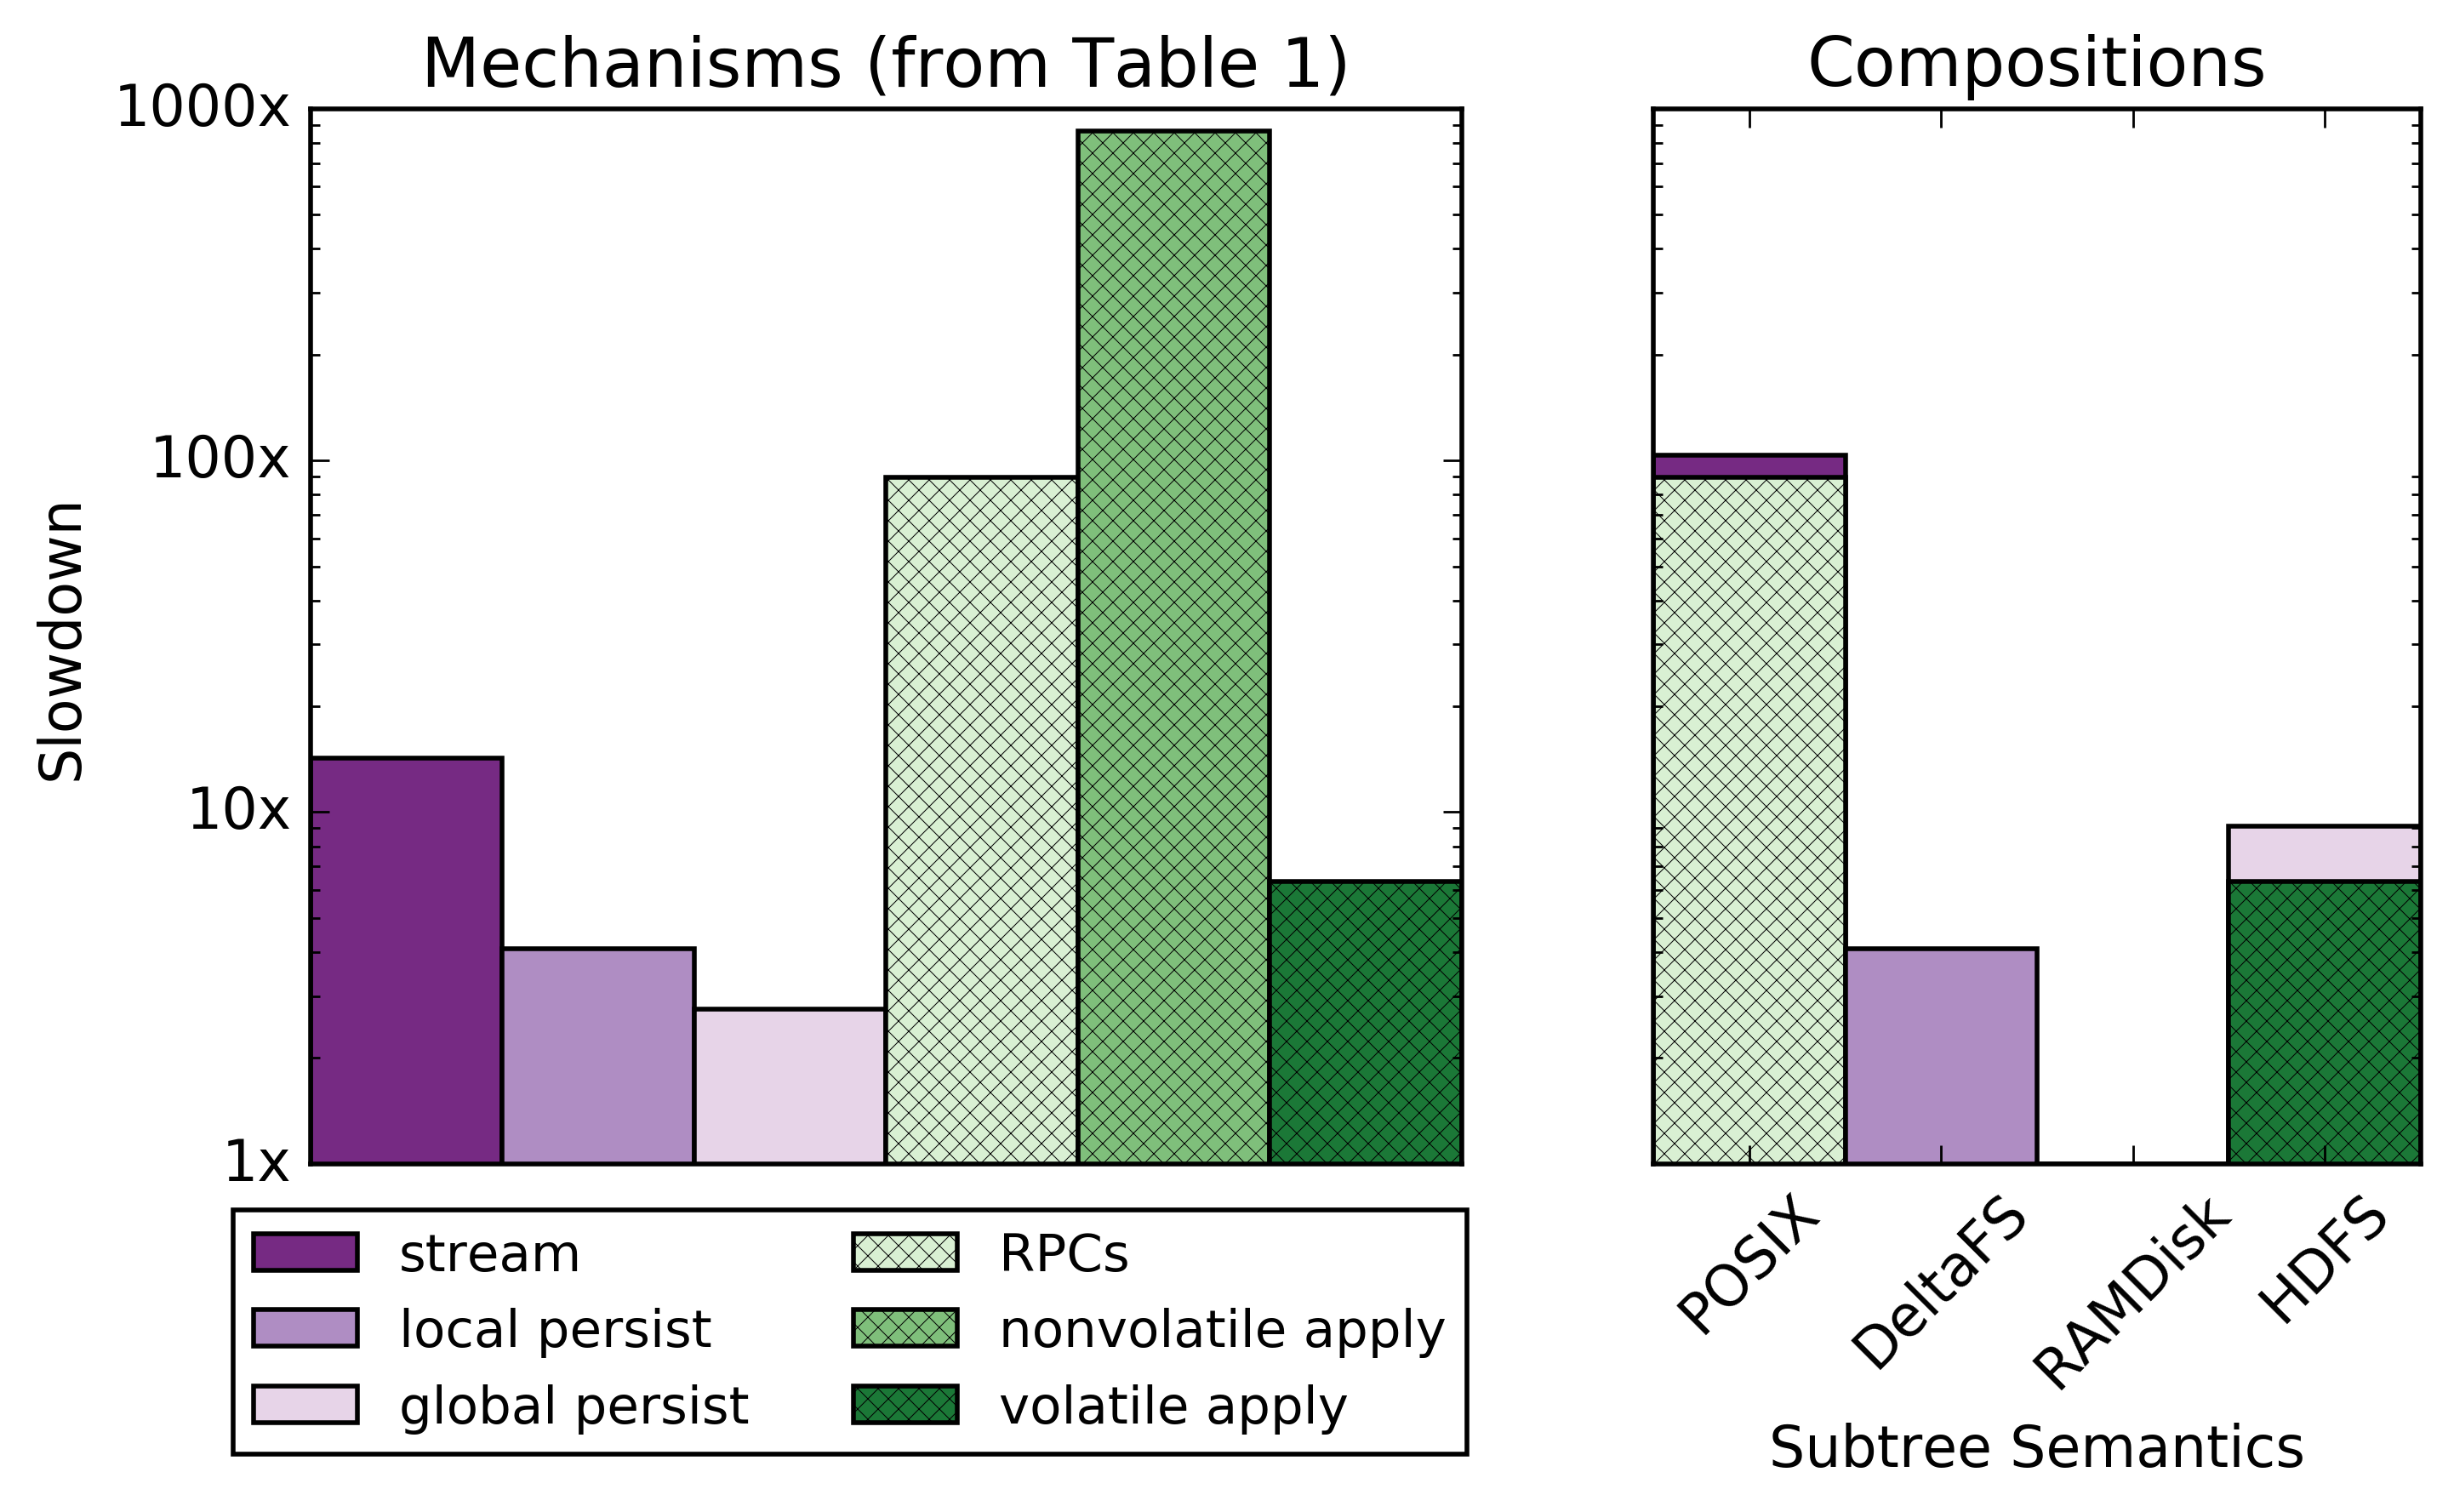
\includegraphics[width=1.0\linewidth]{./chapters/cudele/figures/composable-mechanisms.png}
\caption{Performance of each mechanism (left) and building the
consistency/durability semantics of real-world systems (right) for 100K files
creates from a single client. Results are normalized to the runtime of writing
events to the client's in-memory journal.  \label{fig:composable-mechanisms}}
\end{figure}

%\begin{figure}[tb]
%\centering
%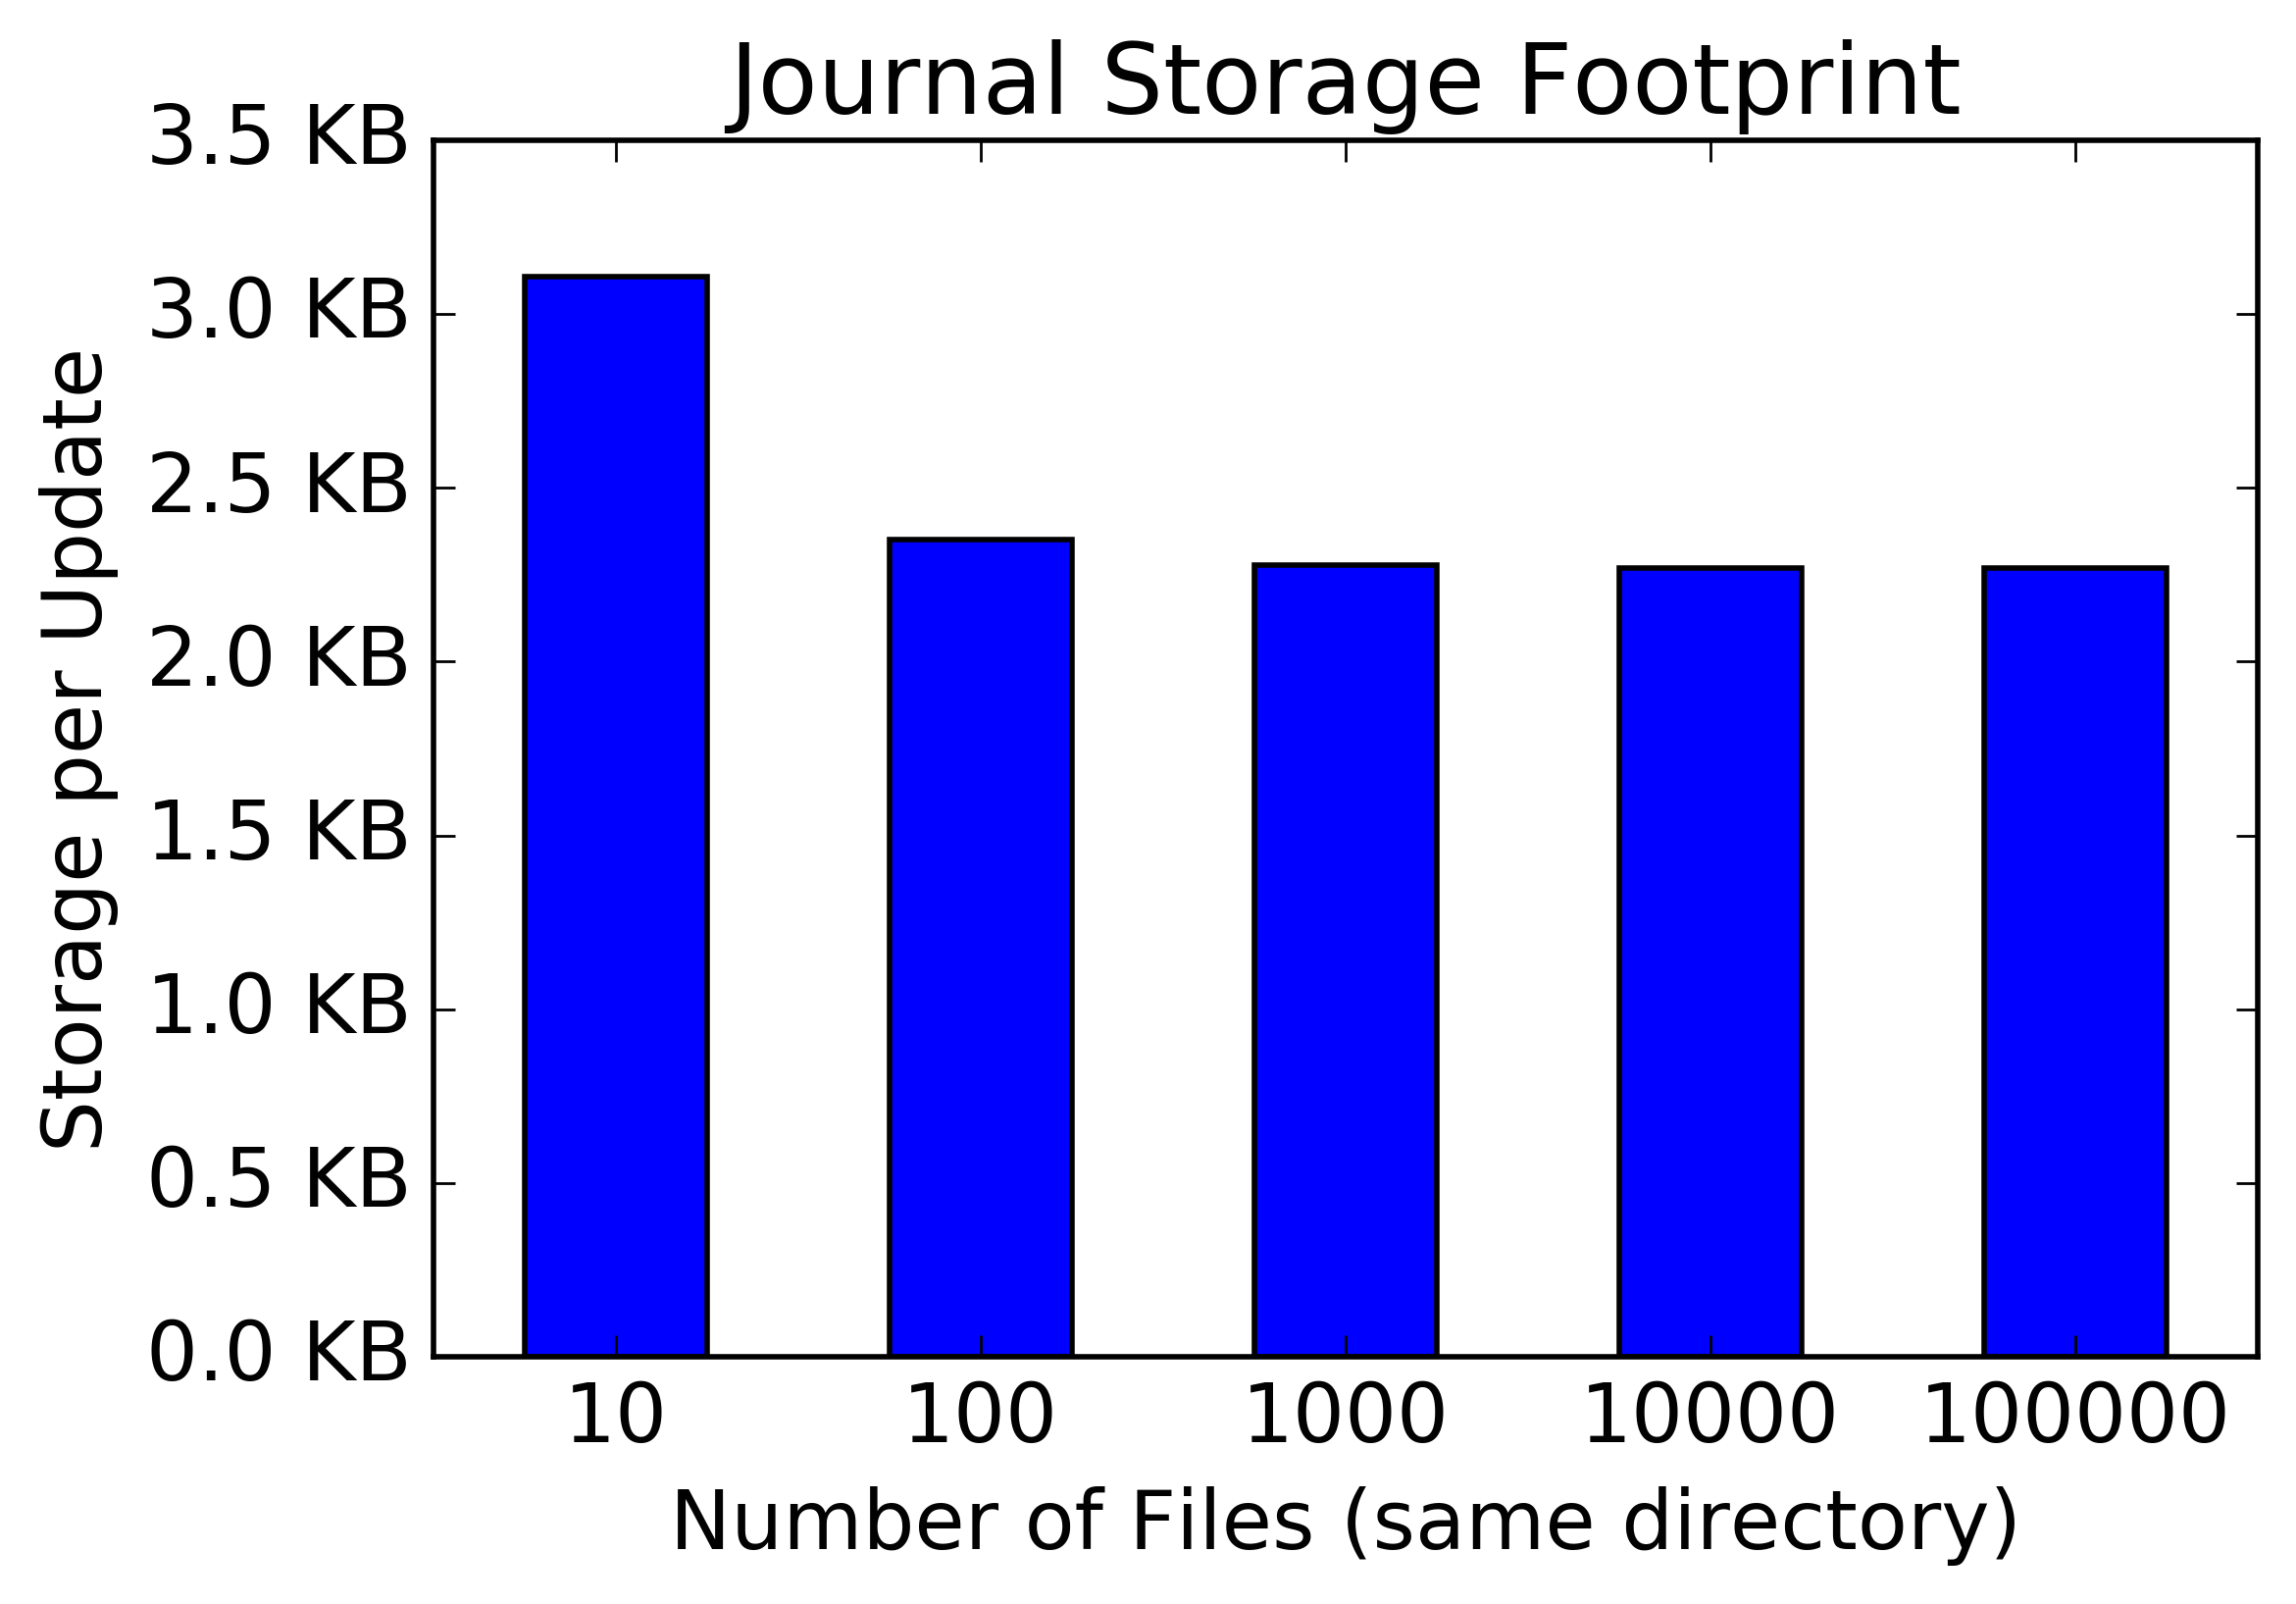
\includegraphics[width=1.0\linewidth]{./chapters/cudele/figures/behavior-journal-size.png}
%\caption{ [\href{https://...}{source}] Microbenchmark: storage footprint on
%client. The size of the client's journal scales with the number of
%updates.\label{fig:behavior-journal-size}}
%\end{figure}

Figure~\ref{fig:composable-mechanisms} shows the runtime of the Cudele
mechanisms for a single client creating files in the same directory, normalized
to the time it takes to write 100K file create updates to the client's
in-memory journal ({\it i.e.} the Append Client Journal mechanism).
Stream is an approximation of the overhead and is calculated by subtracting
the runtime of the job with the journal turned off from the runtime with the
journal turned on.  100K is the maximum recommended size of a directory in
CephFS; preliminary experiments with larger directory sizes show memory
problems.

{\it Poorly Scaling Data Structures:} Despite doing the same amount of work,
mechanisms that rely on poorly scaling data structures have large slowdowns for
the larger number of creates. For example, RPCs has a \(90\times\) slowdown
because it relies on the internal CephFS directory data structures. It is a
well-known problem that directory data structures do not scale when creating
files in the same directory~\cite{ren:sc2014-indexfs} and any mechanism that
uses these data structures will experience similar slowdowns. Other mechanisms
that write events to a journal) experience a much less drastic slowdown because
the journal data structure does not need to be scanned for every operation.
Events are written to the end of the journal without even checking the validity
({\it e.g.}, if the file already exists for a create), which is another form of
relaxed consistency because the file system assumes the application has
resolved conflicting updates in a different way.

% RPCs vs. apply: calls to metadata server vs. RADOS
{\it Overhead of RPCs:} RPCs is \(66\times\) slower than Volatile
Apply because sending individual metadata updates over the network is costly.
While RPCs sends a request for every file create, Volatile Apply
writes all the updates to the in-memory journal and applies them to the
in-memory data structures in the metadata server. While communicating the
decoupled namespace directly to the metadata server is faster, communicating
through the object store (Nonvolatile Apply) is \(10\times\) slower.

% TODO: why is apply so slow.  
% apply: no CephFS changes, pulls/pushes same RADOS obj.
% v_apply vs. apply/persist: communicating through RADOS
{\it Overhead of Nonvolatile Apply:} The cost of Nonvolatile
Apply is much larger than all the other mechanisms.  That mechanism was not
implemented as part of Cudele -- it was a debugging and recovery tool packaged
with CephFS. It works by iterating over the updates in the journal and pulling
all objects that {\it may} be affected by the update.  This means that two
objects are repeatedly pulled, updated, and pushed: the object that houses the
experiment directory and the object that contains the root directory ({\it
i.e.} \texttt{/}).  The cost of communicating through the object store is shown
by comparing the runtime of Volatile Apply + Global Persist to
Nonvolatile Apply. These two operations end up with the same final metadata
state but using Nonvolatile Apply is clearly inferior.

% persist vs. save: one disk vs. many
{\it Parallelism of the Object Store:} Comparing Local and Global
Persist demonstrates the bandwidth advantages of storing the journal in a
distributed object store. The Global Persist
performance is \(1.5\times\) faster because the object store is leveraging the
collective bandwidth of the disks in the cluster. This benefit comes from the
object store itself but should be acknowledged when making decisions for the
application; the bandwidth of the object store can help mitigate the overheads of
globally persisting metadata updates.

{\it Journal Size:} We measure the amount of storage per journal update to be
about 2.5\text{KB}. The storage footprint scales linearly with the number of
metadata creates and suggests that updates for a million files would be 2.5KB
\(*\) 1 million files \(=\) 2.38GB. Transfer times for payloads of this size in
most HPC/data center networks are reasonable.

\textbf{Takeaway}: measuring the mechanisms individually shows that their
overheads and costs can differ {\it by orders of magnitude}. We also show that
some mechanisms, like Nonvolatile Apply, are not worthwhile as currently
implemented.

\subsection{Use Case 1: Creates in the Same Directory}
\label{sec:use-case-1}

\begin{figure*}[t]
  \centering
  \begin{subfigure}[b]{.3\linewidth}
      \centering
      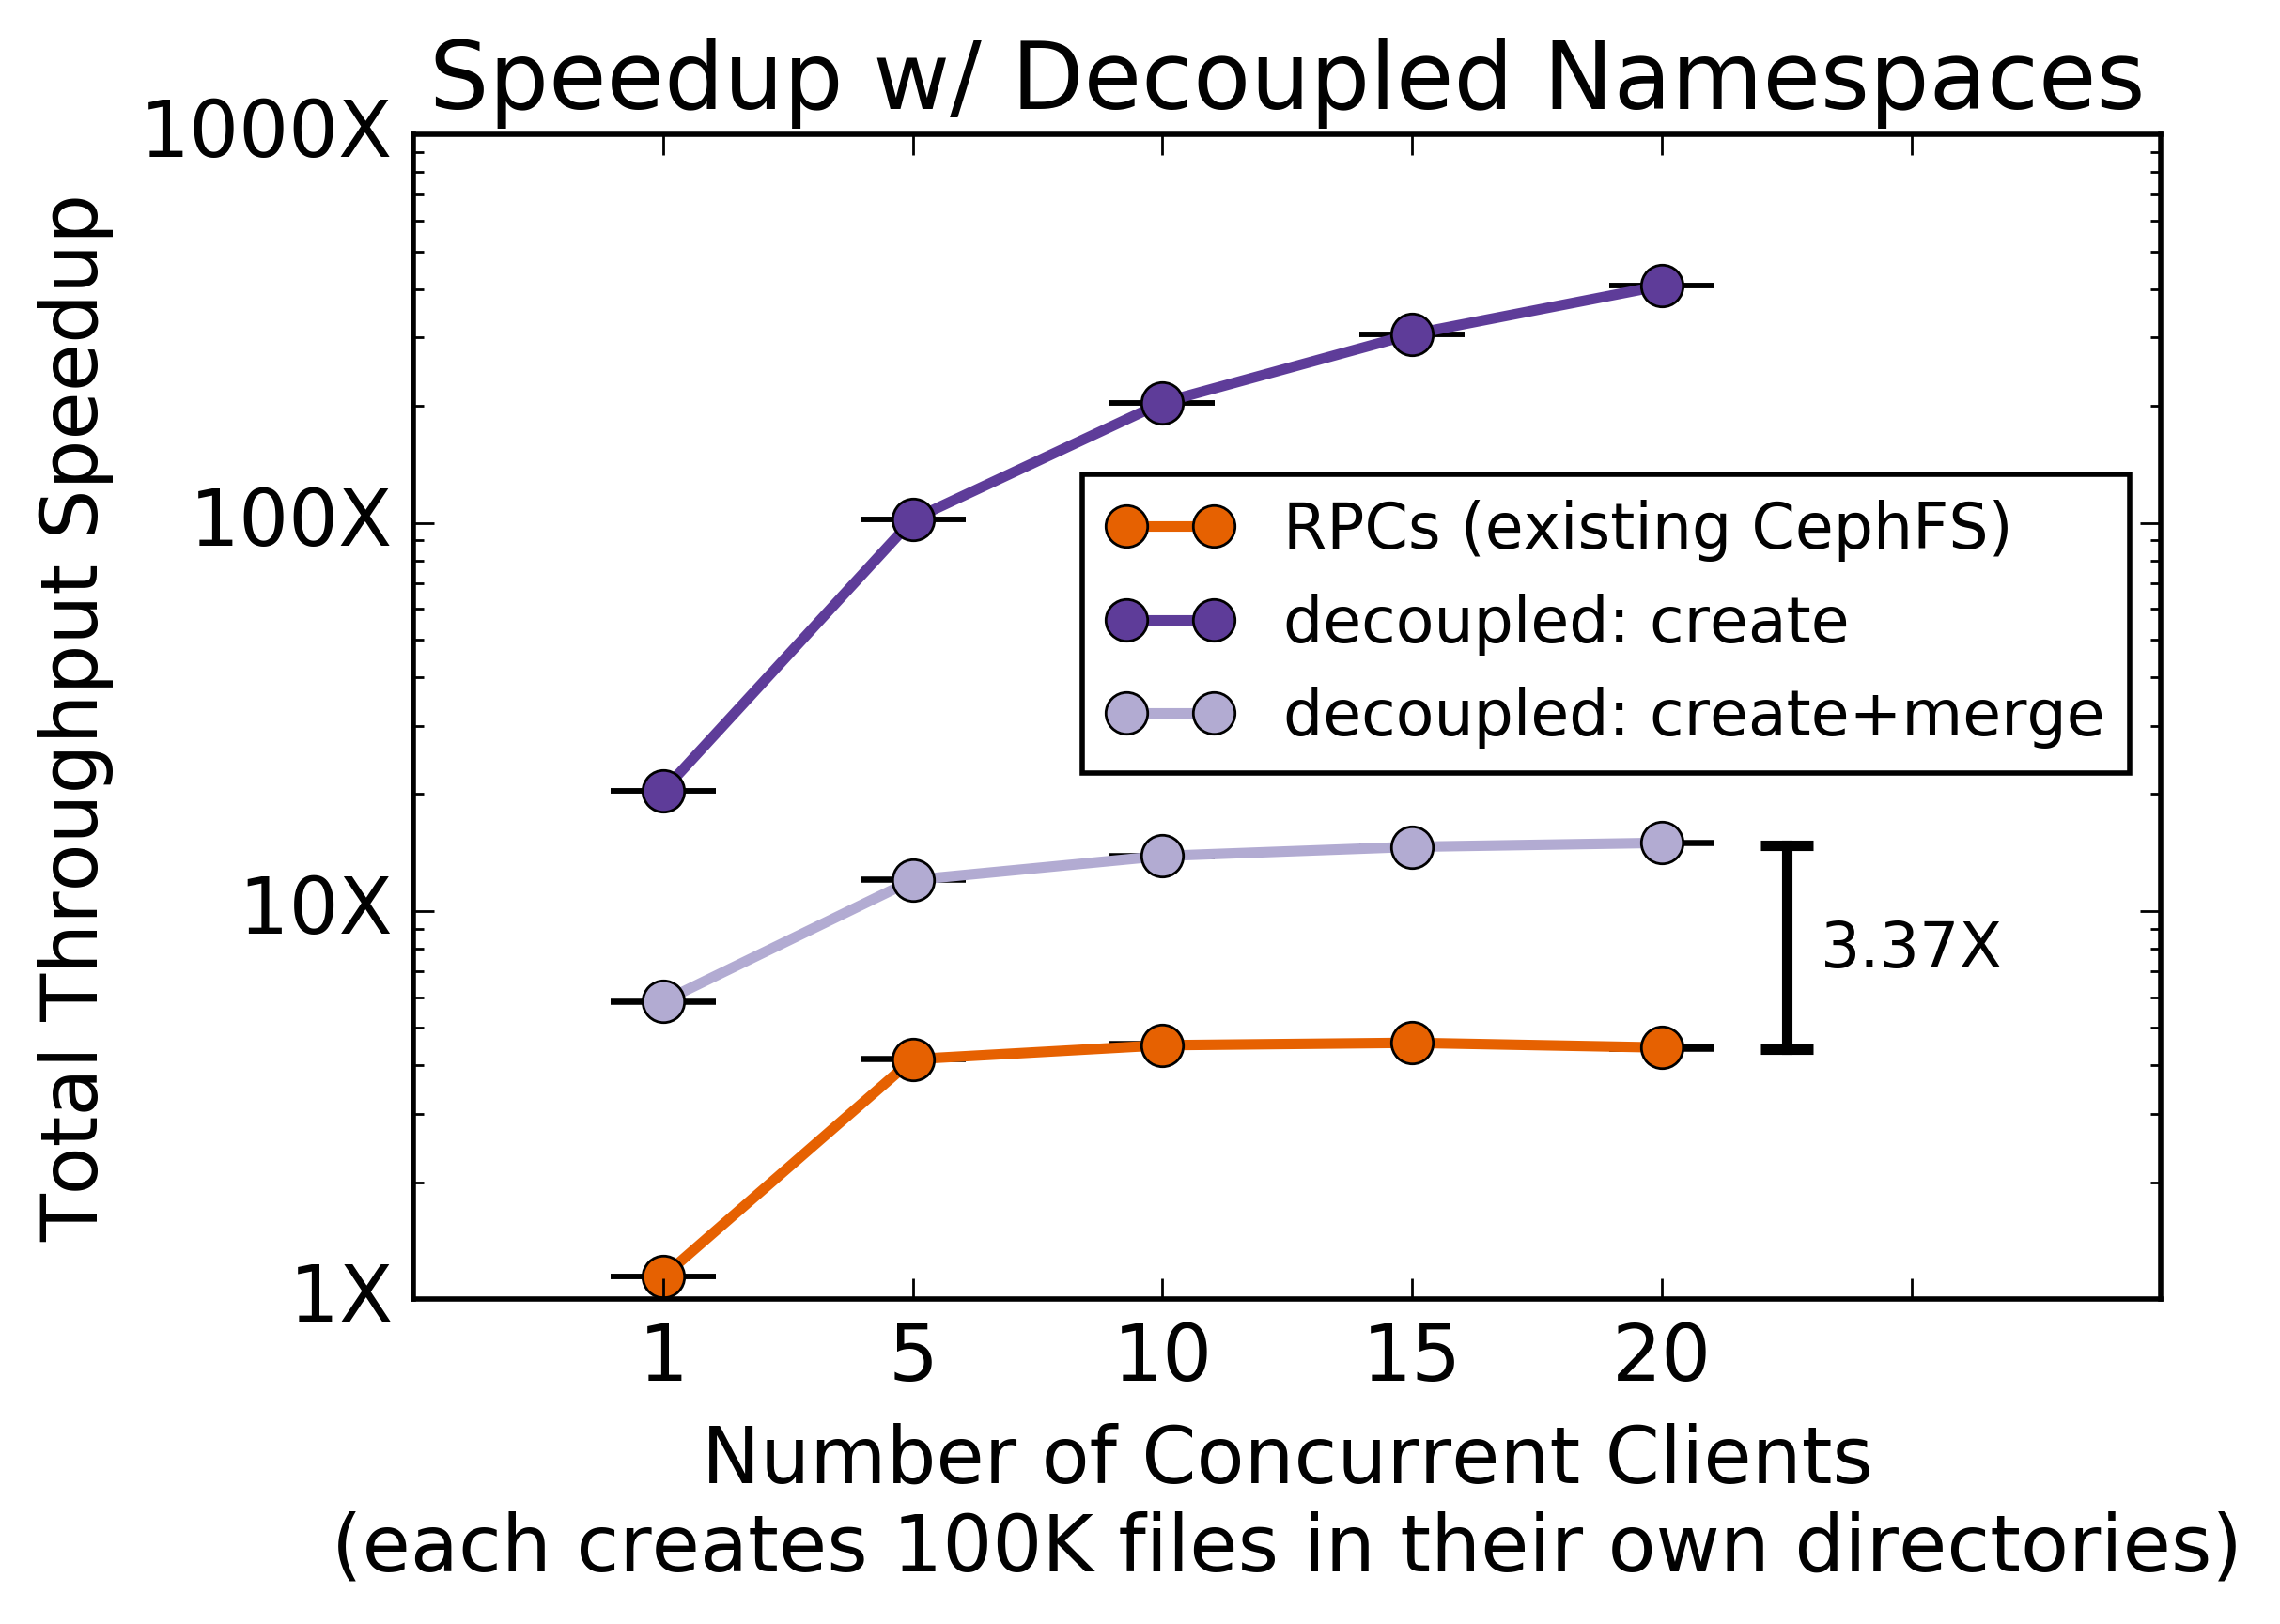
\includegraphics[width=1.0\linewidth]{./chapters/cudele/figures/mergescale.png}
      \caption{Use Case 1} \label{fig:mergescale}
  \end{subfigure}
  \begin{subfigure}[b]{.3\linewidth}
      \centering
      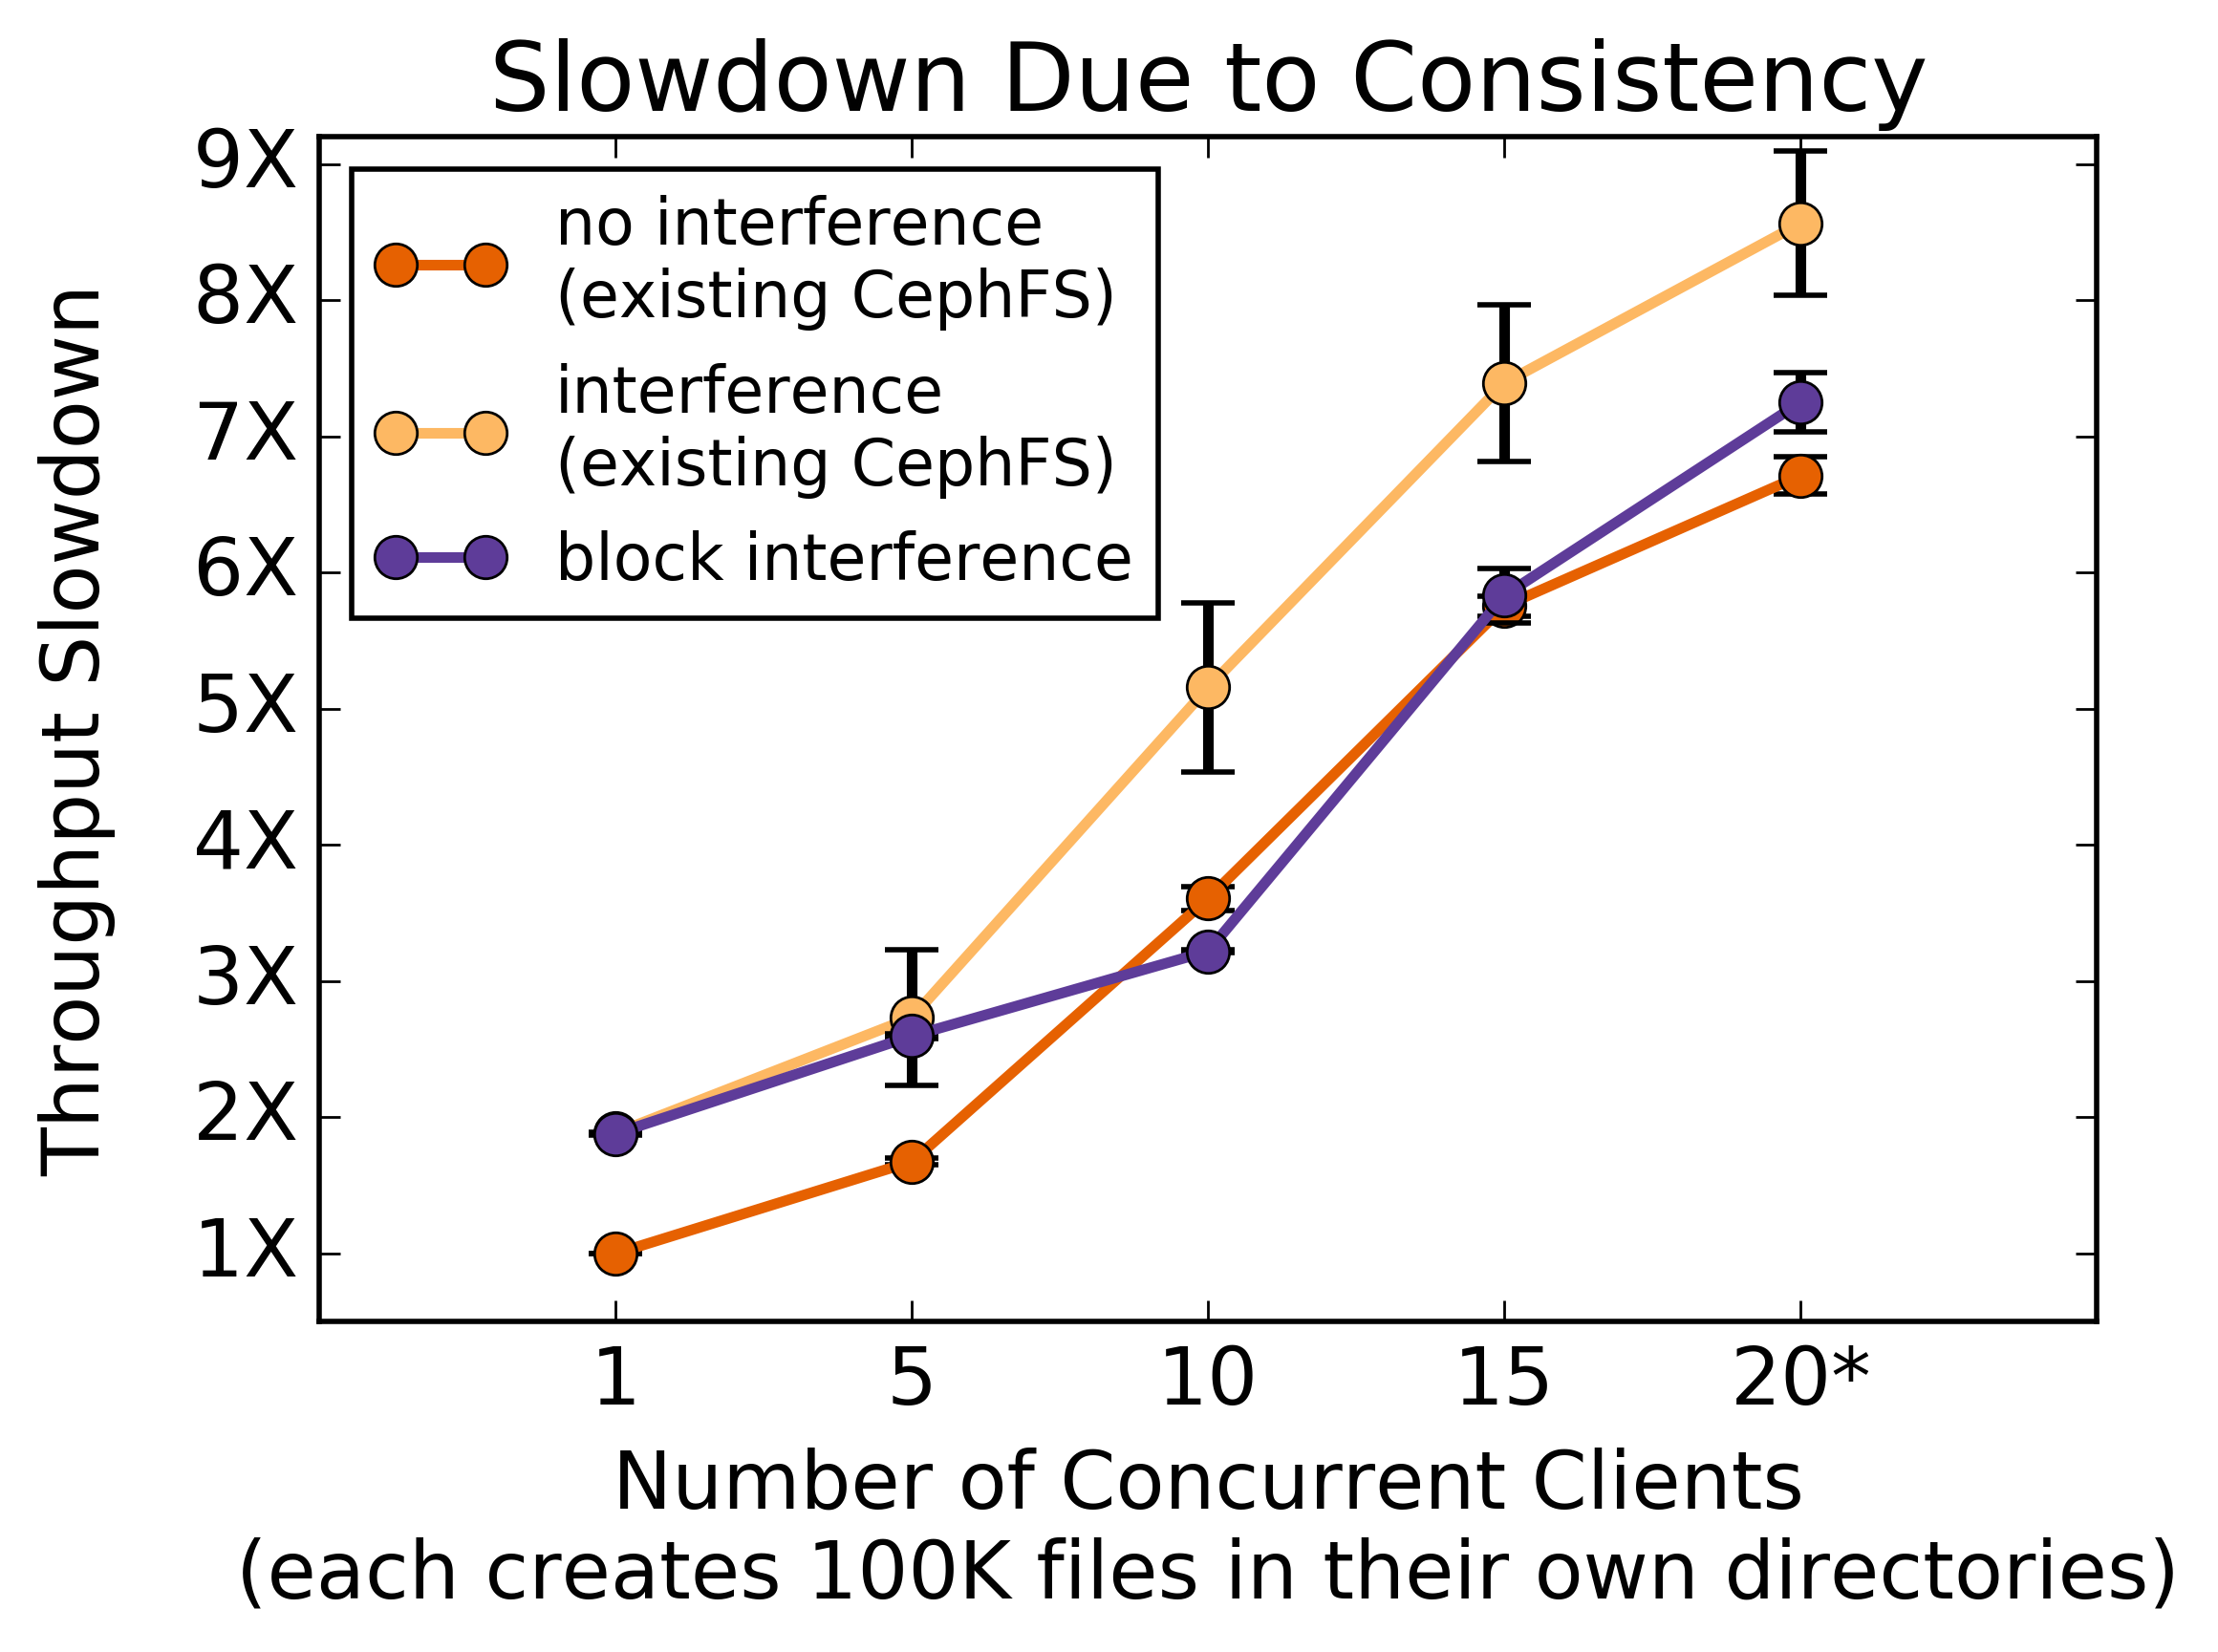
\includegraphics[width=1.0\linewidth]{./chapters/cudele/figures/block-allow.png}
      \caption{Use Case 2}
      \label{fig:block-allow}
  \end{subfigure}
  \begin{subfigure}[b]{.3\linewidth}
      \centering
      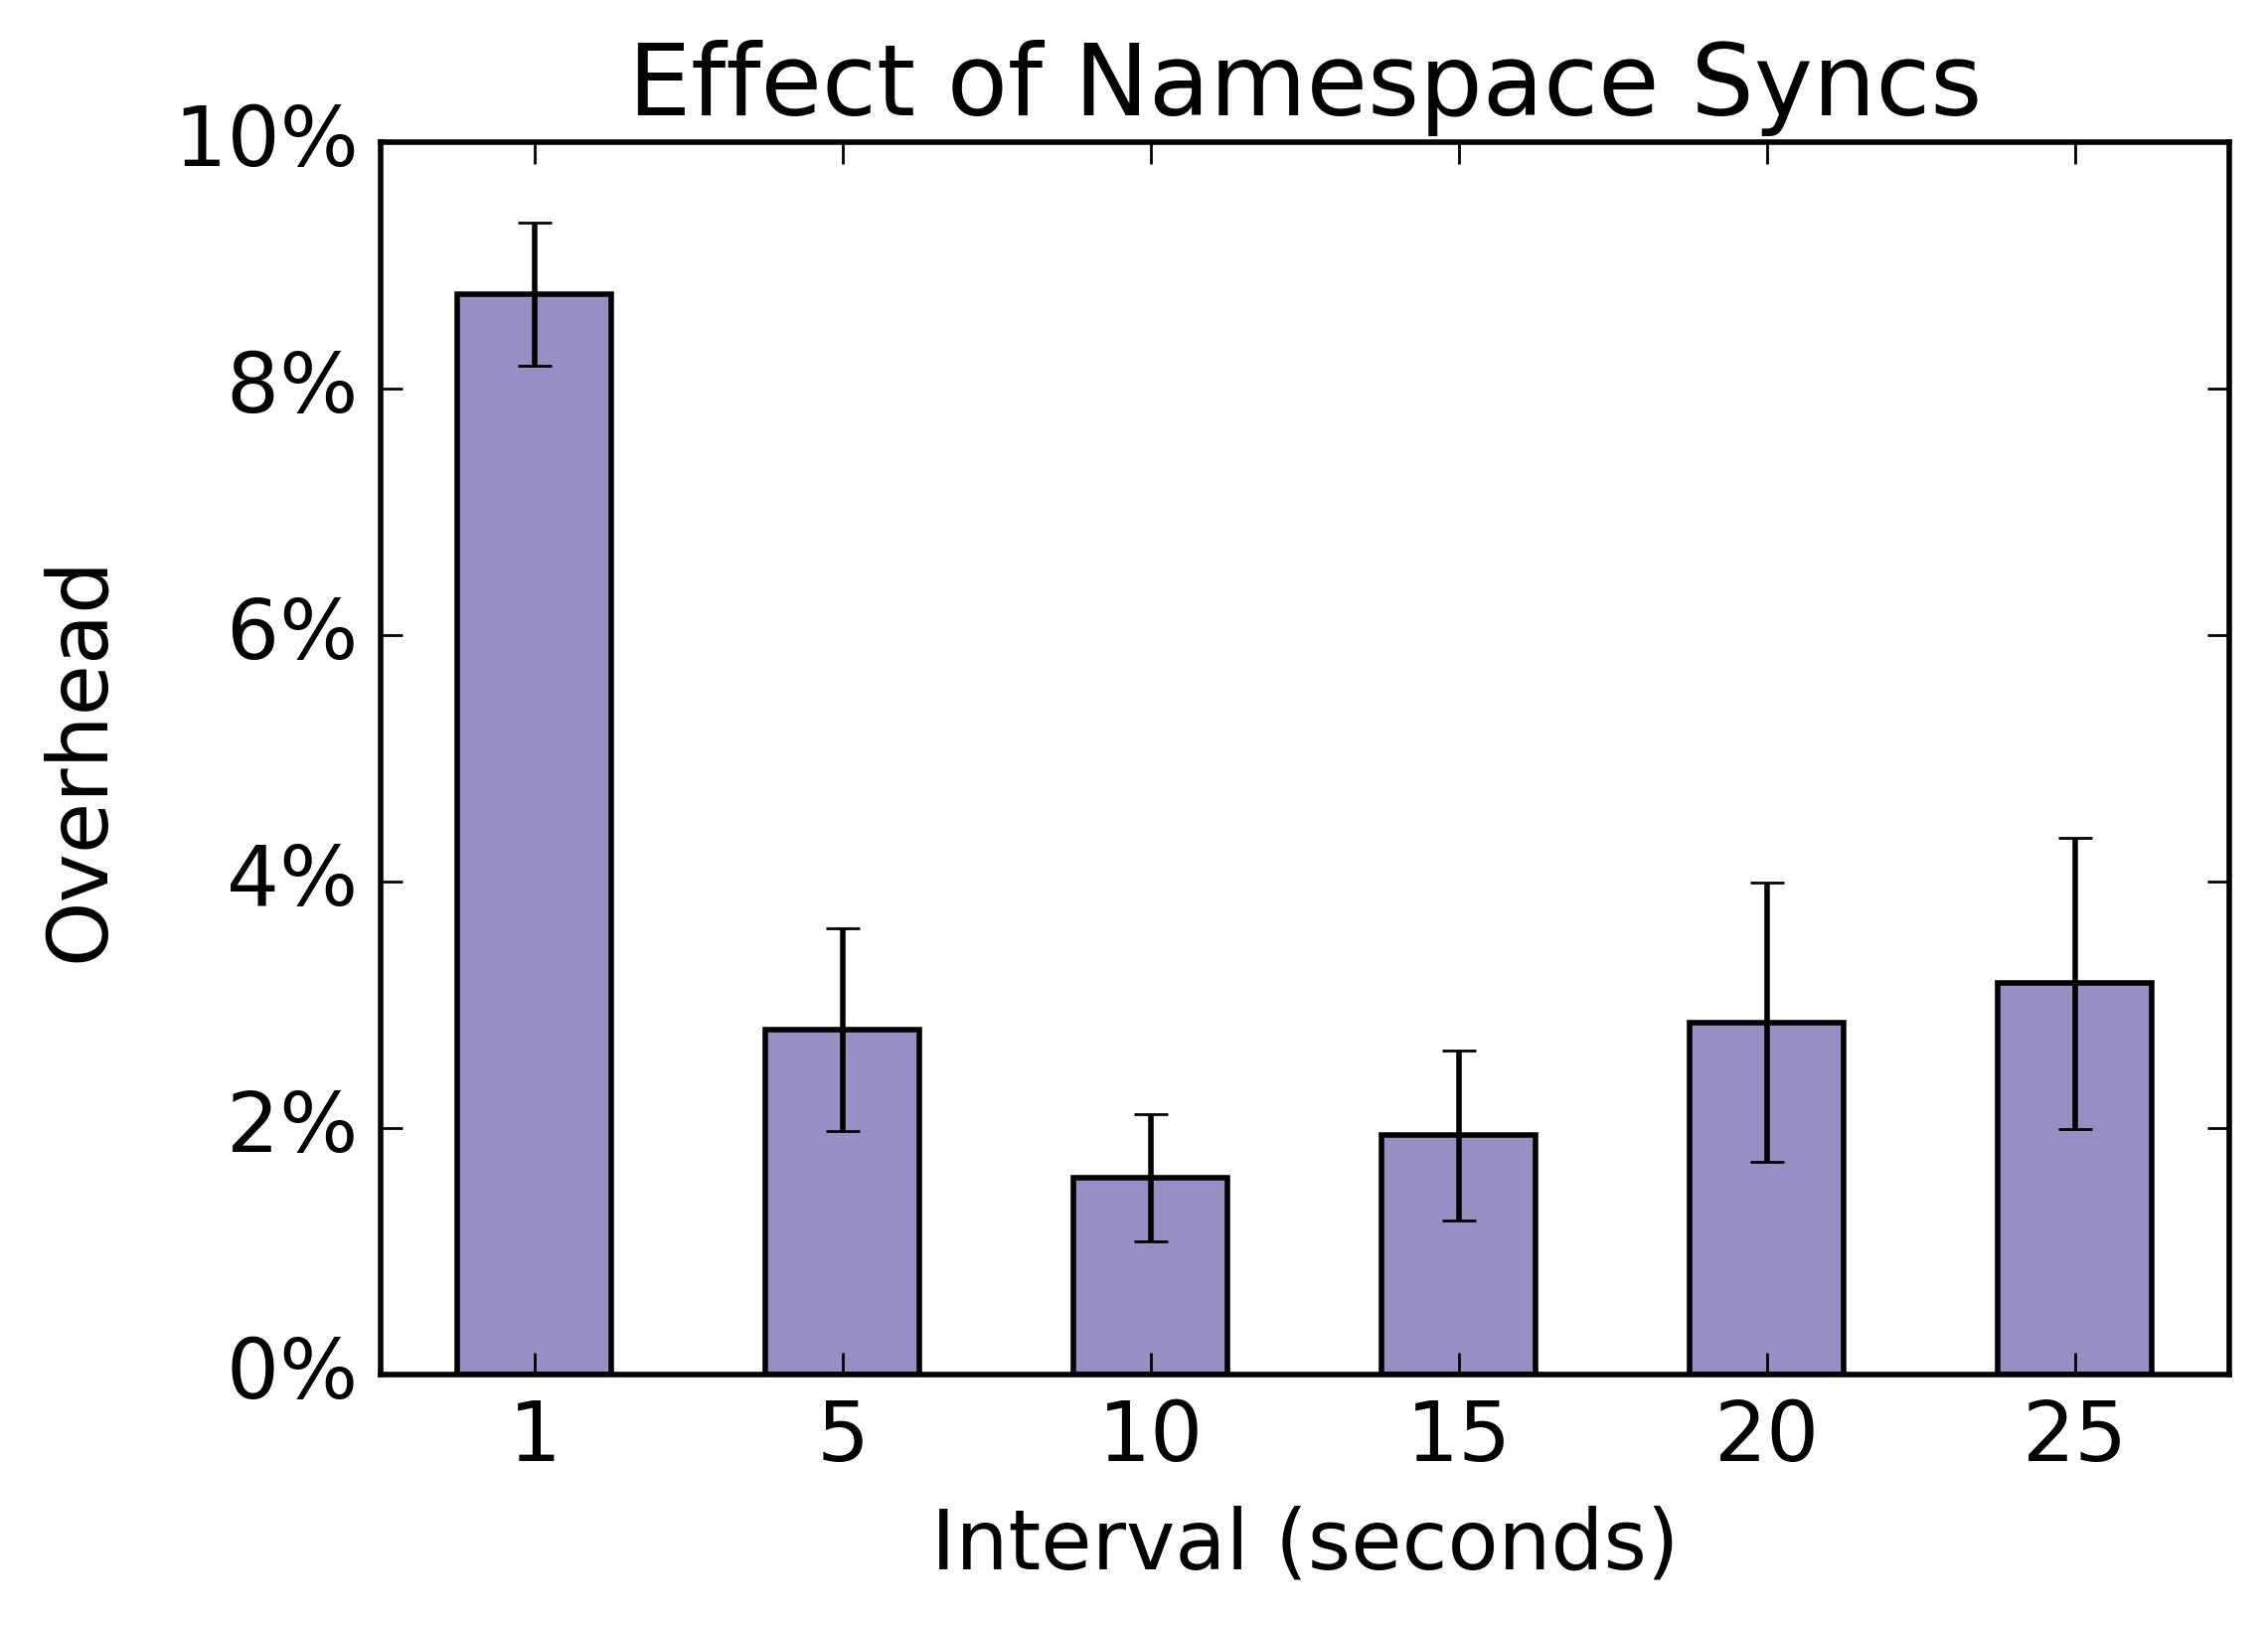
\includegraphics[width=1.0\linewidth]{./chapters/cudele/figures/slowdown-sync.png}
      \caption{Use Case 3}
      \label{fig:slowdown-sync}
  \end{subfigure}
\caption{The performance and features of Cudele. (a) shows the cost of
merging client journals at the metadata server. Shipping and merging journals of updates scales better than RPCs
because there are less messages and consistency/durability code paths are
bypassed. In (b), the allow/block API isolates directories from interfering
clients. (c) is the slowdown of a single client syncing updates to the global
namespace. The inflection point is the trade-off of frequent updates vs. larger
journal files.\label{fig:use-cases}}
\end{figure*}

First we show how we can build application-specific subtrees by composing
mechanisms and that this approach results in more a scalable global namespace.
We start with clients creating files in private directories because this
workload is heavily studied in HPC and appears in other contexts~\ref{RELATED
WORK}.

%\begin{figure}[tb]
%\centering
%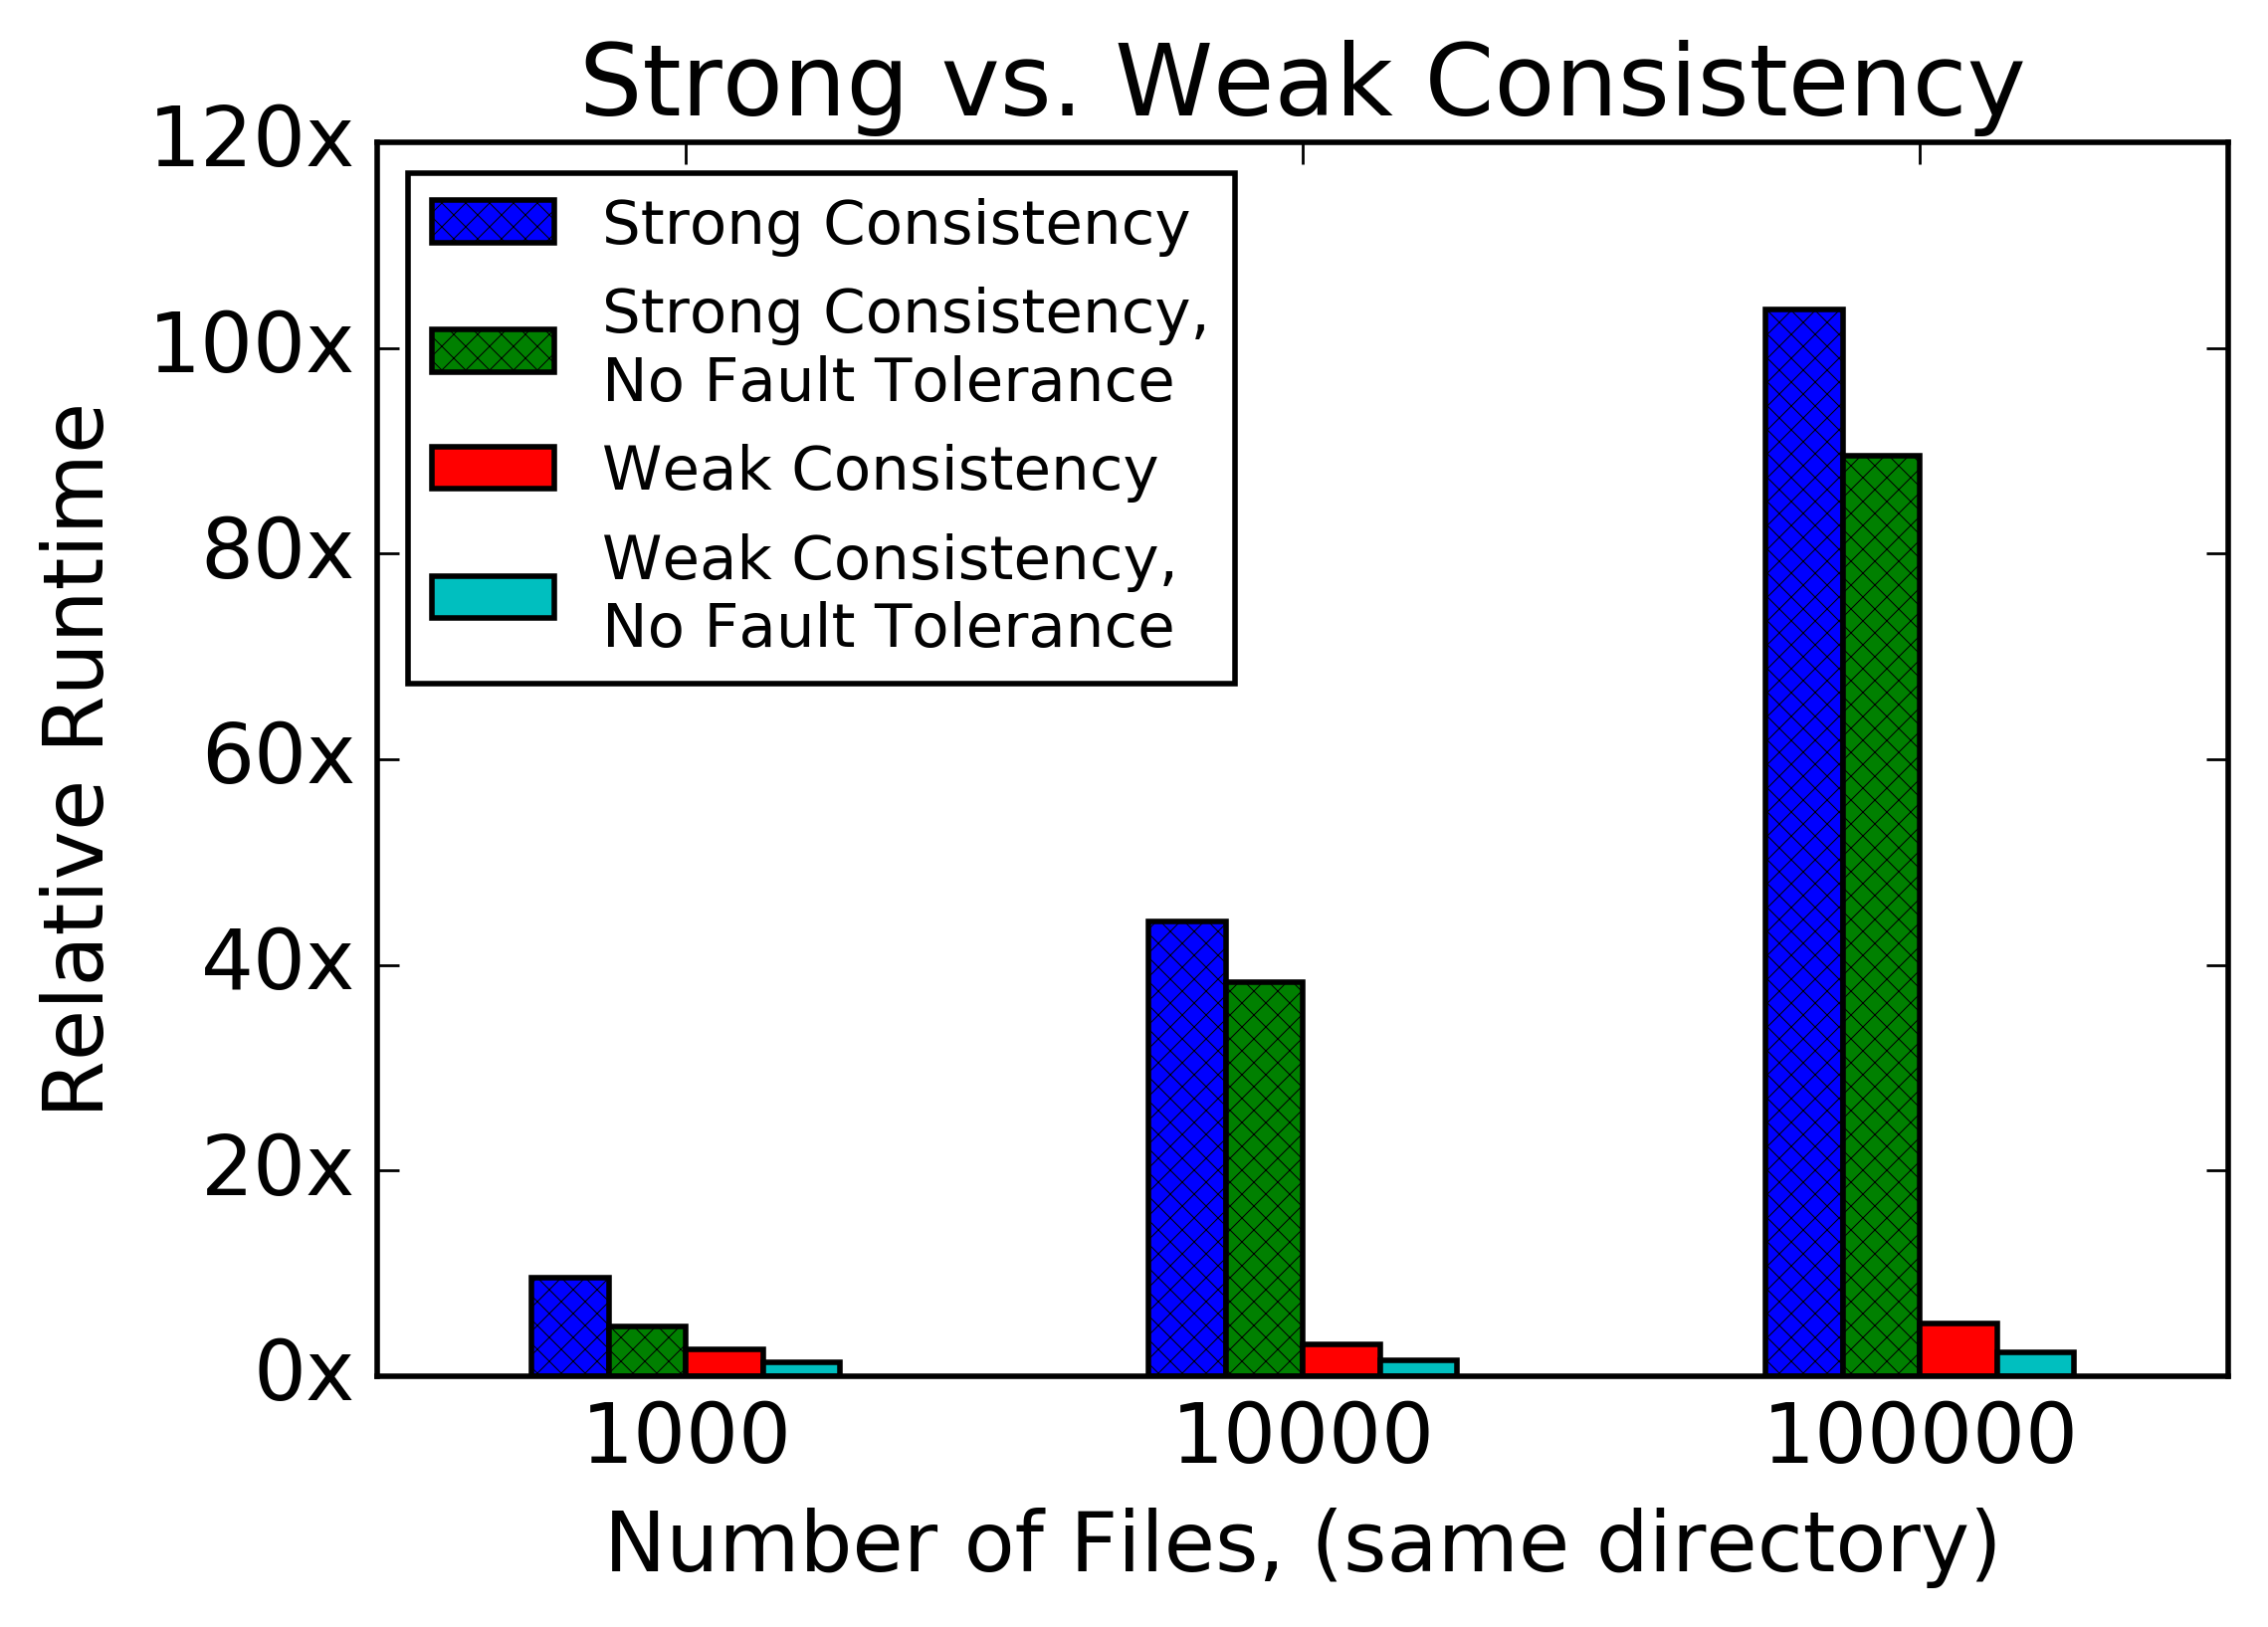
\includegraphics[width=1.0\linewidth]{./chapters/cudele/figures/slowdown-strong-v-weak.png}
%\caption{ [\href{https://...}{source}] Use Case 1: the RPC per metadata update
%(strong consistency) has a large overhead compared to decoupled namespaces
%(weak consistency.)\label{fig:slowdown-strong-weak}}
%\end{figure}

The graph on the right of Figure~\ref{fig:composable-mechanisms} shows how
applications can compose mechanisms together to get the consistency/durability
guarantees they need in a global namespace.  We label the \(x\)-axis with
systems that employ these semantics, as described in
Figure~\ref{fig:subtree-policies}.  Again, the runtime is normalized to
creating files in the client's in-memory journal.  We make no guarantees
during execution of the mechanisms or when transitioning semantics -- the
semantics are guaranteed {\it once the mechanism completes}. So if servers fail
during a mechanism, metadata or data may be lost.

\textbf{Takeaway}: we confirm the performance benefits of other
well-established research systems but, more importantly, we show that the
Cudele mechanisms we propose are useful for building and evaluating different
consistency/durability semantics.\\

To show the contention at the metadata server, in Figure~\ref{fig:mergescale}
we scale the number of clients for the RPC per operation strategy and the
decoupled namespace strategy. For RPCs, we increase the number of clients
making requests to the metadata server and for decoupled (the merge bars), we
increase the number of concurrent journal merge requests. So for the 30 clients
data point, we are measuring the operations per second for 30 client journals
that land on the metadata server at the same time. The ``create \& merge" bar
adds the time it takes for clients to generate the journal of events in
parallel. The experiment is run three times but the standard deviation is too
small to see.

%Merge requests are serialized at the metadata server; merging concurrently is
%an optimization for future work. The current implementation has race conditions
%because the metadata server recovery code was not designed to run in parallel
%({\it i.e.} the metadata server never recovers with multiple threads). As a
%result, the metadata server versions inodes and directory entries to ensure
%that the recovered metadata is consistent.

This workload scales further with decoupled namespaces because the metadata
server is not overwhelmed with RPC requests. Compared to
Figure~\ref{fig:overhead-c} we can scale to 40 clients which is more than
double the capacity of a single metadata server using the RPC strategy to
maintain strong consistency. Related work has pointed to on-disk metadata
format as the primary factor for improved scalability; but our results show
that the weakened consistency and durability enables the scalability
improvements. The on-disk metadata formats in this experiment are the same for
all schemes.

The performance of decoupled namespaces is better than RPCs because we place no
restrictions on the validity of metadata inserted into the journal and avoid
touching poorly scaling data structures. We can scale linearly if we weaken our
consistency by never checking for the existence of files before creating files
({\it i.e.} only append \texttt{open()} requests to the journal).  When the
updates are merged by the metadata server into the in-memory metadata store
they never scan growing data structures.  Had we implemented the Append Client
Journal mechanism to include \texttt{lookup()} commands before \texttt{open()}
requests, we would have seen the poor scaling that we see with the RPCs
mechanism. 

%% DeltaFS vs. BatchFS vs. POSIX IO: decoupled is faster
%% (5-7x) vs. (90-104x) slower
%% Does not scale?
%% Strong Consistency > 10X slower than Weak Consistency 
%{\it Speedups of Decoupled Namespaces:} Weak consistency uses the
%decoupled namespace strategy and shows up to a \(20\times\) speedup over the
%traditional namespaces that use RPCs. Compared to the baseline the slowdown is
%\(5-7\times\) for Strong Consistency, which emulates BatchFS and
%\(90-104\times\) for Weak Consistency, which emulates DeltaFS.

%{\it Durability \(<<\) Consistency:} The performance of these semantics
%suggests that the overhead of consistency is much larger than the overhead of
%durability. This conclusion should be stronger as we scale the number of files
%because the cost of streaming the journal into the object store is constant.
%
% Weak Consistency benefit not due to metadata format

\textbf{Takeaway}: the ability to couple well-established techniques to
specific applications allows the global namespace to scale further and perform
better. In our case, RPCs overwhelm the system but decoupling/shipping a
journal of updates improves scalability by 2\(\times\).

%\section{notes}
%Linking clients into our custom libcephfs
%
%Use namespace's recursive data structure to put policies on subtrees
%- consistency: weak vs. strong, global vs. local
%  - e.g., BatchFS/DeltaFS: weak, local
%  - e.g., POSIX IO: strong, global
%  - e.g., PLFS: no consistency
%- durability: global vs. local
%  - e.g., CephFS: global
%  - e.g., BatchFS/DeltaFS: local
%
%Experimental Setup
%- Ceph: 9 OSDs, 1 metadata server, 2 kernel client
%- Workload limitations: blah
%
%Workload: creates
%
%Baseline: 200K creates in the same directory
%- throughput: degrades at 950s
%- CPU utilization: more at 950s
%- inode cache: eviction dominate
%- inodes +- to cache: eviction dominate
%- per-disk throughput: RADOS not bottleneck
%
%Experiment 1: Interference
%
%\subsection{Baseline}
%Experiment 0: creates in the same directory
%- setup: why we use caching, we use the kernel client, how we circumvent max fragment size
%
%Experiment 0: creates with a stat
%- Hypothesis: metadata read pauses creates and requires a snapshot in time
%  - what is more of an overhead: pausing creates and getting a consistent view OR sucking up resources as it reads from RADOS?
%- can we delay snapshot?
%
%Experiment 1: creates with a readdir
%- Hypothesis: shows the cost of synchronization because on a write, the first client drops his caps
%- client0: create 100k, client1: stat at 2 mins
%
%Experiment 2: scale the number of files
%- See if the open/close spike occurs 
%- Try to see why open/close spike is allowed to happen
%- Try to disable all caching -- metadata writes don't ever re-use the inode -- we never ask for it again!
%- client0: create 100k, client1: touch at 2 mins
%
%Experiment 3: see how fast the cache satisfies a read
%- client0: create 100k, stat inodes
%- client0: create 100k, client1: stat inodes
%
%lient 0: creates, client 1 create(s)

\subsection{Use Case 2: Creates with Interfering Client}

Next we show how Cudele can be programmed to block interfering clients using
the same problematic workload from Figure~\ref{fig:overhead-b}. In this
workload, clients create files in private directories and a separate client
interferes by creating more files in each directory. This introduces false
sharing and the metadata server revokes capabilities on directories touched by
the interfering client. While HPC tries to avoid these situations with
workflows~\cite{zheng:pdsw2014-batchfs, zheng:pdsw2015-deltafs}, it still
happens in distributed file systems when users unintentionally access
directories in a shared file system.  We only scale to 15 clients because the
performance variability of a nearly overloaded metadata server, in our case 18
clients, is too high.

Figure~\ref{fig:block-allow} plots the overhead of the slowest client and the
error bars are the standard deviation of 3 runs.  ``Interfere (Fig 3c)" is the
result from Figure~\ref{fig:overhead-b}; ``Interfere" uses the allow/block API
to return \texttt{-EBUSY} to interfering clients; and ``Isolated" is the
baseline performance without an interfering. Each subtree has RPCs and
Stream enabled.  Results are normalized to the runtime of a single
client creating files in a directory. Note that IndexFS has a similar behavior
to ``interfere" with leases, except clients block. 

We draw three conclusions: (1) clients that use the API to block interfering
clients  get the same performance as isolated clients, (2) there is a
negligible effect on performance for the extra work the metadata server does to
return \texttt{-EBUSY}, and (3) merging updates from the decoupled client has a
negligible effect on performance.

\textbf{Takeaway}: the API lets users isolate directories when applications
need better and more reliable performance. Blocking updates is an effective way of
controlling consistency.

\subsection{Use Case 3: Read while Writing}

The final use case shows how the API gives users fine-grained control of the
consistency semantics. The use case is recursively listing files or
directories, motivated by~\ref{RELATED WOKR}.

% Does this implementation need to be described in the implementation?
Figure~\ref{fig:slowdown-sync} shows the performance degradation of a single
client writing updates to a decoupled namespace and pausing to send updates to
the metadata server. The error bars are the standard deviations of 3 runs. We
scale the namespace sync interval to show the trade-off of frequently pausing
or writing large logs of updates.  We use an idle core to log the updates and
to do the network transfer. The client only pauses to fork off a background
process, which is expensive as the address space needs to copied. The
alternative is to pause the client completely and write the update to disk but
since this implementation is limited by the speed of the disk, we choose the
memory-to-memory copy of the fork approach.

\textbf{Takeaway}: syncing namespace updates has up to a 9\% overhead and can
be tuned depending on the users preference but, more importantly, the API gives
users fine-grain control of their consistency/durability to support current
practices or experimental workflows.

%\subsection{Use Case 4: Reading Large Directories} 
%
%% CITEME
%The final use case is reading large directories. At job completion, scientists
%might use \texttt{ls} again to see the results. This causes great strain on the
%file system as paths need to traversed and the entire directory, with all its
%entries, must be transferred back to the client. Here we show how decoupling a
%large namespace and materializing the view in memory on the client is faster
%than doing RPCs for walks of the file system namespace.
%
%FigureX shows how fast a client can materialize decoupled namespaces in memory.
%This takes the on-disk file system metadata format and parses them into events
%that can be manipulated and appended to. Again, we scale the number of up

\subsection{Discussion and Future Work}

Cudele and the experiments we present here prompt many avenues for future work.
First is quantifying the benefits of dynamically changing the semantics of a
subtree from stronger to weaker guarantees (or vice versa), as described in the
introduction. Second is embeddable policies, where child subtrees have
specialized features but still maintain the guarantees  of their parent
subtrees. We already show how applications can compose guarantees and control
their performance, knobs that we did not have before, but embeddable policies
are a way to compose the policies themselves.  For example, a RAMDisk subtree
is POSIX IO-compliant but relaxes durability constraints, so it can reside
under a POSIX IO subtree that is strongly consistent. These embeddable policies
should be controlled and enforced by Cudele.  Finally, performance prediction
benefits from our cost quantification of each mechanism. Applications can use
Cudele to microbenchmark their components and software, similar to what we did
in Section~\S\ref{sec:microbenchmarks}. Using those results, they can predict
how much slower their system will be if they adopt stronger consistency or
durability.  This is a form of co-design that takes a ``dirty-slate" approach
but building just the guarantees the application needs from existing
implementations.  This can also be a verification tool where performance that
varies wildly from the predicted performance can be a red flag that something
is wrong or that the bottleneck is not in the consistency or durability plane.

%Second is the opportunity for adding hardware in strategic places to speed up
%the mechanisms that the application needs. In Figure~\ref{fig:mergescale} the
%performance of merging updates at the metadata server is limited by the speed
%of the disk. So applications that rely on merging many updates should consider
%equipping the metadata server with SSDs or more memory. 
%

